\chapter{Исследования}

\section{Предварительное описание}

Проведем тестирование программы на работоспособность сначала для уравнения $-\frac{1}{\mu_0} \Delta A_{\varphi} + \frac{1}{\mu_0} A_{\varphi} = f$, затем на уравнения $-\frac{1}{\mu_0} \Delta A_{\varphi} + \frac{1}{\mu_0 r^2} A_{\varphi} = f$, где $f$ - любая функция, достаточно очевидная для проверки результата. После этого рассмотрим интересующее нас уравнение $-\frac{1}{\mu_0} \Delta A_{\varphi} + \frac{1}{\mu_0 r^2} A_{\varphi} = J_{\varphi}$. Кольцо, создающее поле, расположено в точке $(10; 0)$ и отмечено на рисунке синей точкой. Базисные функции билинейные.  Образец расчетной области изображен на рисунке \ref{fig:exampleOfArea}:

\begin{figure}
	\centering
	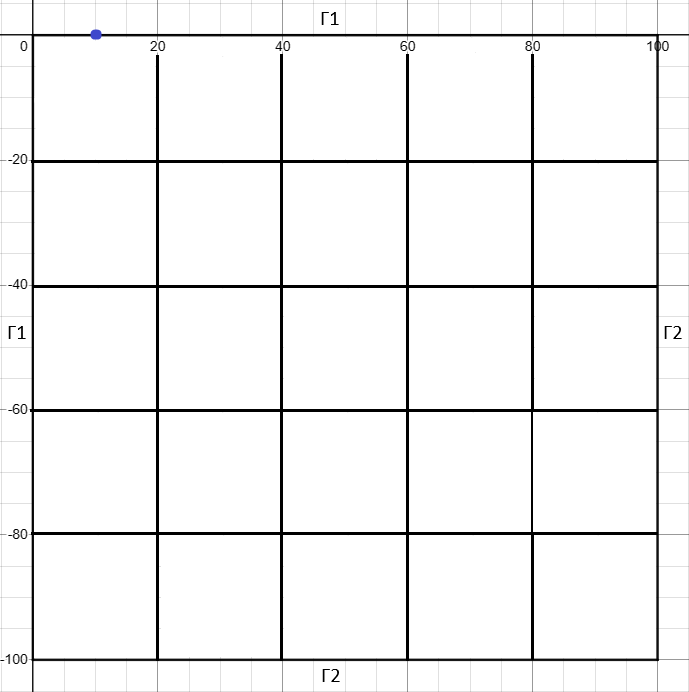
\includegraphics[width=0.75\linewidth]{images/Тест1.png}
	\caption{Расчетная область}
	\label{fig:exampleOfArea}
\end{figure}

\section{Тестирование на работоспособность}

Пусть искомая функция будет $u = r * z$, а  $\mu_0 = 1$, однородные условия первого рода расположены на верхней и левой границах расчетной области, на правой и нижней границе условия однородные второго рода. Получим следующее. 

\begin{table}
	\caption{Тестирование при $-\frac{1}{\mu_0} \Delta A_{\varphi} + \frac{1}{\mu_0} A_{\varphi} = f$, $u = rz$, $f = rz$, $\mu_0 = 1$}
	\centering
	\small
	\begin{tabularx}{1.0\textwidth}{| >{\raggedright\arraybackslash}X | >{\raggedright\arraybackslash}X | >{\raggedright\arraybackslash}X |>{\raggedright\arraybackslash}X |}
		\hline
		\centering{Узел} & \centering{Значение} & \centering{Абсолютная погрешность} & \centering{Относительная погрешность} \tabularnewline \hline
		
		

		\centering{(20,0008; -20)} & \centering{-3.99991668E+002}& \centering{2.43321134E-002} & \centering{6.08278503E-005} \tabularnewline \hline
		\centering{(40,0006; -20)} & \centering{-8.00041536E+002} & \centering{2.95364092E-002} & \centering{3.69199577E-005} \tabularnewline \hline
 		 \centering{(60,0004; -20)} & \centering{-1.19973146E+003} & \centering{2.76538286E-001} & \centering{2.30447035E-004} \tabularnewline \hline
		\centering{(80,0002; -20)} & \centering{-1.60083585E+003} & \centering{8.31847171E-001} & \centering{5.19903182E-004} \tabularnewline \hline
		\centering{(100; -20)} & \centering{-1.99651310E+003} & \centering{3.48690361E+000} & \centering{1.74345181E-003} \tabularnewline \hline


		\centering{(20,0008; -40)} & \centering{-8.00073346E+002}& \centering{4.13461873E-002} & \centering{5.16806669E-005} \tabularnewline \hline
		\centering{(40,0006; -40)} & \centering{-1.60026312E+003} & \centering{2.39123420E-001} & \centering{1.49449896E-004} \tabularnewline \hline
 		\centering{(60,0004; -40)} & \centering{-2.39973286E+003} & \centering{2.83136319E-001} & \centering{1.17972680E-004} \tabularnewline \hline
		\centering{(80,0002; -40)} & \centering{-3.20203212E+003} & \centering{2.02411646E+000} & \centering{6.32534811E-004} \tabularnewline \hline
		\centering{(100; -40)} & \centering{-3.99347480E+003} & \centering{6.52519957E+000} & \centering{1.63129989E-003} \tabularnewline \hline

		\centering{(20,0008; -60)} & \centering{-1.19978676E+003}& \centering{2.61241225E-001} & \centering{2.17692313E-004} \tabularnewline \hline
		\centering{(40,0006; -60)} & \centering{-2.39974806E+003} & \centering{2.87944345E-001} & \centering{1.19975011E-004} \tabularnewline \hline
		\centering{(60,0004; -60)} & \centering{-3.59862984E+003} & \centering{1.39415571E+000} & \centering{3.87262893E-004} \tabularnewline \hline
		\centering{(80,0002; -60)} & \centering{-4.80175375E+003} & \centering{1.74174814E+000} & \centering{3.62863288E-004} \tabularnewline \hline
		\centering{(100; -60)} & \centering{-5.98860115E+003} & \centering{1.13988464E+001} & \centering{1.89980774E-003} \tabularnewline \hline
		 		
		 \centering{(20,0008; -80)} & \centering{-1.60091687E+003}& \centering{8.52871444E-001} & \centering{5.33023331E-004} \tabularnewline \hline
		 \centering{(40,0006; -80)} & \centering{-3.20206687E+003} & \centering{2.01886922E+000} & \centering{6.30887168E-004} \tabularnewline \hline
 		 \centering{(60,0004; -80)} & \centering{-4.80177546E+003} & \centering{1.74346432E+000} & \centering{3.63219313E-004} \tabularnewline \hline
		 \centering{(80,0002; -80)} & \centering{-6.40714832E+003} & \centering{7.13231677E+000} & \centering{1.11442171E-003} \tabularnewline \hline
		 \centering{(100; -80)} & \centering{-7.99078772E+003} & \centering{9.21228366E+000} & \centering{1.15153546E-003} \tabularnewline \hline
		 
		 \centering{(20,0008; -100)} & \centering{-1.99661901E+003}& \centering{3.46099134E+000} & \centering{1.73042645E-003} \tabularnewline \hline
		 \centering{(40,0006; -100)} & \centering{-3.99352786E+003} & \centering{6.53213746E+000} & \centering{1.63300987E-003} \tabularnewline \hline
  		 \centering{(60,0004; -100)} & \centering{-5.98864281E+003} & \centering{1.13971859E+001} & \centering{1.89951832E-003} \tabularnewline \hline
		 \centering{(80,0002; -100)} & \centering{-9.96592479E+003} & \centering{9.21283395E+000} & \centering{1.15160136E-003} \tabularnewline \hline
		 \centering{(100; -100)} & \centering{-9.96592479E+003} & \centering{3.40752140E+001} & \centering{3.40752140E-003} \tabularnewline \hline
		 
 	\end{tabularx}
	\label{tab:test1}
\end{table}

Исходя из приведенных результатов в таблице \ref{tab:test1}, делаем вывод, что программа работает верно.

\newpage

Теперь протестируем программу для уравнения $-\frac{1}{\mu_0} \Delta A_{\varphi} + \frac{1}{\mu_0 r^2} A_{\varphi} = f$. Пусть искомая функция все также будет $u = rz$, тогда $f = \frac{z}{r}$, а  $\mu_0 = 1$, однородные условия первого рода расположены на верхней и левой границах расчетной области, на правой и нижней границе условия однородные второго рода. Получим следующее.  

\begin{table}
	\caption{Тестирование при $-\frac{1}{\mu_0} \Delta A_{\varphi} + \frac{1}{\mu_0 r^2} A_{\varphi} = f$, $u = rz$, $f = \frac{z}{r}$, $\mu_0 = 1$}
	\centering
	\small
	\begin{tabularx}{1.0\textwidth}{| >{\raggedright\arraybackslash}X | >{\raggedright\arraybackslash}X | >{\raggedright\arraybackslash}X |>{\raggedright\arraybackslash}X |}
		\hline
		\centering{Узел} & \centering{Значение} & \centering{Абсолютная погрешность} & \centering{Относительная погрешность} \tabularnewline \hline
		
		
		
		\centering{(20,0008; -20)} & \centering{-5.30195216E+003}& \centering{4.90193616E+003} & \centering{1.22543502E+001} \tabularnewline \hline
		\centering{(40,0006; -20)} & \centering{1.38386203E+003} & \centering{2.18387403E+003} & \centering{2.72980159E+000} \tabularnewline \hline
		\centering{(60,0004; -20)} & \centering{-3.63322442E+002} & \centering{8.36685558E+002} & \centering{6.97233316E-001} \tabularnewline \hline
		\centering{(80,0002; -20)} & \centering{1.00509320E+002} & \centering{1.70051332E+003} & \centering{1.06281817E+000} \tabularnewline \hline
		\centering{(100; -20)} & \centering{-4.94549306E+001} & \centering{1.95054507E+003} & \centering{9.75272535E-001} \tabularnewline \hline
		
		
		\centering{(20,0008; -40)} & \centering{-1.06050859E+004}& \centering{9.80505388E+003} & \centering{-1.22558271E+001} \tabularnewline \hline
		\centering{(40,0006; -40)} & \centering{2.76802513E+003} & \centering{4.36804913E+003} & \centering{2.72998975E+000} \tabularnewline \hline
		\centering{(60,0004; -40)} & \centering{-7.26721979E+002} & \centering{1.67329402E+003} & \centering{6.97201194E-001} \tabularnewline \hline
		\centering{(80,0002; -40)} & \centering{2.01039370E+002} & \centering{3.40104737E+003} & \centering{1.06282465E+000} \tabularnewline \hline
		\centering{(100; -40)} & \centering{-9.89198385E+001} & \centering{3.90108016E+003} & \centering{-9.75270040E-001} \tabularnewline \hline
		
		\centering{(20,0008; -60)} & \centering{-1.59033866E+004}& \centering{1.47033386E+004} & \centering{1.22522921E+001} \tabularnewline \hline
		\centering{(40,0006; -60)} & \centering{4.15095747E+003} & \centering{6.55099347E+003} & \centering{2.72953967E+000} \tabularnewline \hline
		\centering{(60,0004; -60)} & \centering{-1.08980656E+003} & \centering{2.51021744E+003} & \centering{6.97277974E-001} \tabularnewline \hline
		\centering{(80,0002; -60)} & \centering{3.01484793E+002} & \centering{5.10149679E+003} & \centering{1.06280917E+000} \tabularnewline \hline
		\centering{(100; -60)} & \centering{-1.48344038E+002} & \centering{5.85165596E+003} & \centering{9.75275994E-001} \tabularnewline \hline
		
		\centering{(20,0008; -80)} & \centering{-2.12202745E+004}& \centering{1.96202105E+004} & \centering{1.22621411E+001} \tabularnewline \hline
		\centering{(40,0006; -80)} & \centering{5.53861996E+003} & \centering{8.73866796E+003} & \centering{2.73079278E+000} \tabularnewline \hline
		\centering{(60,0004; -80)} & \centering{-1.45410075E+003} & \centering{3.34593125E+003} & \centering{6.97064363E-001} \tabularnewline \hline
		\centering{(80,0002; -80)} & \centering{4.02254968E+002} & \centering{6.80227097E+003} & \centering{1.06285218E+000} \tabularnewline \hline
		\centering{(100; -80)} & \centering{-1.97924358E+002} & \centering{7.80207564E+003} & \centering{9.75259455E-001} \tabularnewline \hline
		
		\centering{(20,0008; -100)} & \centering{-2.64659667E+004}& \centering{2.44658867E+004} & \centering{1.22324541E+001} \tabularnewline \hline
		\centering{(40,0006; -100)} & \centering{6.90817680E+003} & \centering{1.09082368E+004} & \centering{2.72701830E+000} \tabularnewline \hline
		\centering{(60,0004; -100)} & \centering{-1.81376823E+003} & \centering{4.18627177E+003} & \centering{6.97707310E-001} \tabularnewline \hline
		\centering{(80,0002; -100)} & \centering{5.01783996E+002} & \centering{8.50180400E+003} & \centering{1.06272284E+000} \tabularnewline \hline
		\centering{(100; -100)} & \centering{-2.46908390E+002} & \centering{9.75309161E+003} & \centering{9.75309161E-001} \tabularnewline \hline
		
	\end{tabularx}
	\label{tab:test2b}
\end{table}



\newpage

Теперь протестируем программу для уравнения \ref{eq1M} для нулевого слоя по времени. $J_{\varphi}$ - $\delta$-функция, равная 1 при $(r, z) = (10, 0)$ и 0 во всех остальных точках. Сетка изображена на рисунке \ref{fig:exampleOfArea}. Однородные краевые условия первого рода находятся на правой и нижней границе, однородные второго рода на верхней и левой границах. Таким образом получим следующее. 


\begin{table}
	\caption{Тестирование исходной функции}
	\centering
	\small
	\begin{tabularx}{1.0\textwidth}{| >{\raggedright\arraybackslash}X |
	>{\raggedright\arraybackslash}X |}
		\hline
		\centering{Узел} & \centering{Значение} \tabularnewline \hline
		
		
		\centering{(0,001; 0)} & \centering{9.89596002E+000} \tabularnewline \hline
		
		\centering{(20,0008; 0)} & \centering{4.59762041E+000}
		\tabularnewline \hline
		
		\centering{(40,0006; 0)} & \centering{2.05043455E+000} \tabularnewline \hline
		
		\centering{(60,0004; 0)} & \centering{1.04570134E+000}
		\tabularnewline \hline
		
		\centering{(80,0002; 0)} & \centering{4.41814204E-001}
		\tabularnewline \hline
		
		
		\centering{(0,001; -20)} & \centering{6.58639311E-002} \tabularnewline \hline

		\centering{(20,0008; -20)} & \centering{3.00036881E-002}
		\tabularnewline \hline
		
		\centering{(40,0006; -20)} & \centering{1.67783663E-002} \tabularnewline \hline
		
		\centering{(60,0004; -20)} & \centering{9.20512908E-003}
		\tabularnewline \hline
		
		\centering{(80,0002; -20)} & \centering{3.99440695E-003}
		\tabularnewline \hline
		
		
		\centering{(0,001; -40)} & \centering{-1.72040980E-002} \tabularnewline \hline

		\centering{(20,0008; -40)} & \centering{-7.83509188E-003}
		\tabularnewline \hline
		
		\centering{(40,0006; -40)} & \centering{-4.37808675E-003} \tabularnewline \hline
		
		\centering{(60,0004; -40)} & \centering{-2.40083452E-003}
		\tabularnewline \hline
		
		\centering{(80,0002; -40)} & \centering{-1.04159964E-003}
		\tabularnewline \hline
		
		
		\centering{(0,001; -60)} & \centering{4.47563199E-003} \tabularnewline \hline

		\centering{(20,0008; -60)} & \centering{2.03775872E-003}
		\tabularnewline \hline
		
		\centering{(40,0006; -60)} & \centering{1.13777548E-003} \tabularnewline \hline
		
		\centering{(60,0004; -60)} & \centering{6.23635462E-004}
		\tabularnewline \hline
		
		\centering{(80,0002; -60)} & \centering{2.70511050E-004}
		\tabularnewline \hline
		
		
		\centering{(0,001; -80)} & \centering{-1.09467887E-003} \tabularnewline \hline
		
		\centering{(20,0008; -80)} & \centering{-4.98291674E-004}
		\tabularnewline \hline
		
		\centering{(40,0006; -80)} & \centering{-2.78024921E-004} \tabularnewline \hline
		
		\centering{(60,0004; -80)} & \centering{-1.52325956E-004}
		\tabularnewline \hline
		
		\centering{(80,0002; -80)} & \centering{-6.60620166E-005}
		\tabularnewline \hline
		
	\end{tabularx}
	\label{tab:test3b}
\end{table}

Исходя из результатов в таблице \ref{tab:test3b}, интуитивно можно предположить, что результат программы необходимо аппроксимирует решение задачи. 